\documentclass[twoside]{book}

% Packages required by doxygen
\usepackage{calc}
\usepackage{doxygen}
\usepackage{graphicx}
\usepackage[utf8]{inputenc}
\usepackage{makeidx}
\usepackage{multicol}
\usepackage{multirow}
\usepackage{textcomp}
\usepackage[table]{xcolor}

% NLS support packages
\usepackage[T2A]{fontenc}
\usepackage[czech]{babel}

% Font selection
\usepackage[T1]{fontenc}
\usepackage{mathptmx}
\usepackage[scaled=.90]{helvet}
\usepackage{courier}
\usepackage{amssymb}
\usepackage{sectsty}
\renewcommand{\familydefault}{\sfdefault}
\allsectionsfont{%
  \fontseries{bc}\selectfont%
  \color{darkgray}%
}
\renewcommand{\DoxyLabelFont}{%
  \fontseries{bc}\selectfont%
  \color{darkgray}%
}

% Page & text layout
\usepackage{geometry}
\geometry{%
  a4paper,%
  top=2.5cm,%
  bottom=2.5cm,%
  left=2.5cm,%
  right=2.5cm%
}
\tolerance=750
\hfuzz=15pt
\hbadness=750
\setlength{\emergencystretch}{15pt}
\setlength{\parindent}{0cm}
\setlength{\parskip}{0.2cm}
\makeatletter
\renewcommand{\paragraph}{%
  \@startsection{paragraph}{4}{0ex}{-1.0ex}{1.0ex}{%
    \normalfont\normalsize\bfseries\SS@parafont%
  }%
}
\renewcommand{\subparagraph}{%
  \@startsection{subparagraph}{5}{0ex}{-1.0ex}{1.0ex}{%
    \normalfont\normalsize\bfseries\SS@subparafont%
  }%
}
\makeatother

% Headers & footers
\usepackage{fancyhdr}
\pagestyle{fancyplain}
\fancyhead[LE]{\fancyplain{}{\bfseries\thepage}}
\fancyhead[CE]{\fancyplain{}{}}
\fancyhead[RE]{\fancyplain{}{\bfseries\leftmark}}
\fancyhead[LO]{\fancyplain{}{\bfseries\rightmark}}
\fancyhead[CO]{\fancyplain{}{}}
\fancyhead[RO]{\fancyplain{}{\bfseries\thepage}}
\fancyfoot[LE]{\fancyplain{}{}}
\fancyfoot[CE]{\fancyplain{}{}}
\fancyfoot[RE]{\fancyplain{}{\bfseries\scriptsize Generováno po 23. dub 2018 15.\-49\-:34 pro projekt Proj2 I\-V\-S -\/ kalkulacka programem Doxygen }}
\fancyfoot[LO]{\fancyplain{}{\bfseries\scriptsize Generováno po 23. dub 2018 15.\-49\-:34 pro projekt Proj2 I\-V\-S -\/ kalkulacka programem Doxygen }}
\fancyfoot[CO]{\fancyplain{}{}}
\fancyfoot[RO]{\fancyplain{}{}}
\renewcommand{\footrulewidth}{0.4pt}
\renewcommand{\chaptermark}[1]{%
  \markboth{#1}{}%
}
\renewcommand{\sectionmark}[1]{%
  \markright{\thesection\ #1}%
}

% Indices & bibliography
\usepackage{natbib}
\usepackage[titles]{tocloft}
\setcounter{tocdepth}{3}
\setcounter{secnumdepth}{5}
\makeindex

% Hyperlinks (required, but should be loaded last)
\usepackage{ifpdf}
\ifpdf
  \usepackage[pdftex,pagebackref=true]{hyperref}
\else
  \usepackage[ps2pdf,pagebackref=true]{hyperref}
\fi
\hypersetup{%
  colorlinks=true,%
  linkcolor=blue,%
  citecolor=blue,%
  unicode%
}

% Custom commands
\newcommand{\clearemptydoublepage}{%
  \newpage{\pagestyle{empty}\cleardoublepage}%
}


%===== C O N T E N T S =====

\begin{document}

% Titlepage & ToC
\hypersetup{pageanchor=false}
\pagenumbering{roman}
\begin{titlepage}
\vspace*{7cm}
\begin{center}%
{\Large Proj2 I\-V\-S -\/ kalkulacka \\[1ex]\large 2 }\\
\vspace*{1cm}
{\large Generováno programem Doxygen 1.8.6}\\
\vspace*{0.5cm}
{\small po 23. dub 2018 15.49:34}\\
\end{center}
\end{titlepage}
\clearemptydoublepage
\tableofcontents
\clearemptydoublepage
\pagenumbering{arabic}
\hypersetup{pageanchor=true}

%--- Begin generated contents ---
\chapter{Rejstřík prostorů jmen}
\section{Seznam prostorů jmen}
Zde naleznete seznam všech dokumentovaných prostorů jmen se stručným popisem\-:\begin{DoxyCompactList}
\item\contentsline{section}{\hyperlink{namespaceCalculator}{Calculator} }{\pageref{namespaceCalculator}}{}
\end{DoxyCompactList}

\chapter{Rejstřík hierarchie tříd}
\section{Hierarchie tříd}
Zde naleznete seznam, vyjadřující vztah dědičnosti tříd. Je seřazen přibližně (ale ne úplně) podle abecedy\-:\begin{DoxyCompactList}
\item Form\begin{DoxyCompactList}
\item \contentsline{section}{Calculator.\-Calculator\-G\-U\-I}{\pageref{classCalculator_1_1CalculatorGUI}}{}
\end{DoxyCompactList}
\end{DoxyCompactList}

\chapter{Rejstřík tříd}
\section{Seznam tříd}
Následující seznam obsahuje především identifikace tříd, ale nacházejí se zde i další netriviální prvky, jako jsou struktury (struct), unie (union) a rozhraní (interface). V seznamu jsou uvedeny jejich stručné popisy\-:\begin{DoxyCompactList}
\item\contentsline{section}{\hyperlink{classCalculator_1_1CalculatorGUI}{Calculator.\-Calculator\-G\-U\-I} }{\pageref{classCalculator_1_1CalculatorGUI}}{}
\end{DoxyCompactList}

\chapter{Rejstřík souborů}
\section{Seznam souborů}
Zde naleznete seznam všech dokumentovaných souborů se stručnými popisy\-:\begin{DoxyCompactList}
\item\contentsline{section}{\hyperlink{Program_8cs}{Program.\-cs} }{\pageref{Program_8cs}}{}
\end{DoxyCompactList}

\chapter{Dokumentace prostorů jmen}
\hypertarget{namespaceCalculator}{\section{Balík Calculator}
\label{namespaceCalculator}\index{Calculator@{Calculator}}
}
\subsection*{Třídy}
\begin{DoxyCompactItemize}
\item 
class \hyperlink{classCalculator_1_1CalculatorGUI}{Calculator\-G\-U\-I}
\item 
class {\bfseries Program}
\end{DoxyCompactItemize}

\chapter{Dokumentace tříd}
\hypertarget{classCalculator_1_1CalculatorGUI}{\section{Dokumentace třídy Calculator.\-Calculator\-G\-U\-I}
\label{classCalculator_1_1CalculatorGUI}\index{Calculator.\-Calculator\-G\-U\-I@{Calculator.\-Calculator\-G\-U\-I}}
}
Diagram dědičnosti pro třídu Calculator.\-Calculator\-G\-U\-I\begin{figure}[H]
\begin{center}
\leavevmode
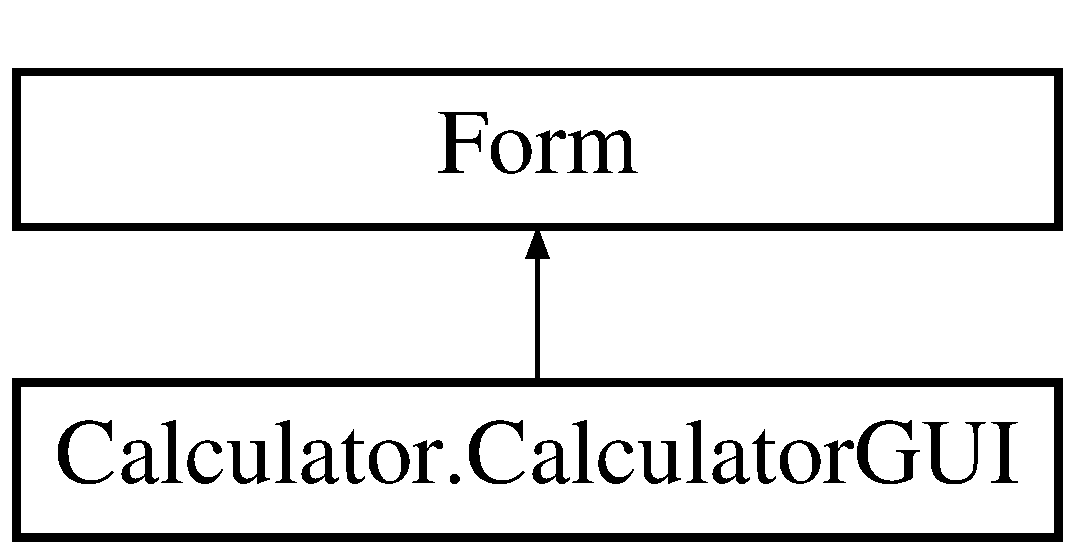
\includegraphics[height=2.000000cm]{classCalculator_1_1CalculatorGUI}
\end{center}
\end{figure}
\subsection*{Chráněné metody}
\begin{DoxyCompactItemize}
\item 
override void \hyperlink{classCalculator_1_1CalculatorGUI_acc8f832b8154c8cba8a80c4e16254d51}{Dispose} (bool disposing)
\begin{DoxyCompactList}\small\item\em Clean up any resources being used. \end{DoxyCompactList}\end{DoxyCompactItemize}


\subsection{Dokumentace k metodám}
\hypertarget{classCalculator_1_1CalculatorGUI_acc8f832b8154c8cba8a80c4e16254d51}{\index{Calculator\-::\-Calculator\-G\-U\-I@{Calculator\-::\-Calculator\-G\-U\-I}!Dispose@{Dispose}}
\index{Dispose@{Dispose}!Calculator::CalculatorGUI@{Calculator\-::\-Calculator\-G\-U\-I}}
\subsubsection[{Dispose}]{\setlength{\rightskip}{0pt plus 5cm}override void Calculator.\-Calculator\-G\-U\-I.\-Dispose (
\begin{DoxyParamCaption}
\item[{bool}]{disposing}
\end{DoxyParamCaption}
)\hspace{0.3cm}{\ttfamily [inline]}, {\ttfamily [protected]}}}\label{classCalculator_1_1CalculatorGUI_acc8f832b8154c8cba8a80c4e16254d51}


Clean up any resources being used. 


\begin{DoxyParams}{Parametry}
{\em disposing} & true if managed resources should be disposed; otherwise, false.\\
\hline
\end{DoxyParams}


Dokumentace pro tuto třídu byla generována z následujících souborů\-:\begin{DoxyCompactItemize}
\item 
Form1.\-cs\item 
Form1.\-Designer.\-cs\end{DoxyCompactItemize}

\chapter{Dokumentace souborů}
\hypertarget{Program_8cs}{\section{Dokumentace souboru Program.\-cs}
\label{Program_8cs}\index{Program.\-cs@{Program.\-cs}}
}
\subsection*{Třídy}
\begin{DoxyCompactItemize}
\item 
class {\bfseries Calculator.\-Program}
\end{DoxyCompactItemize}
\subsection*{Prostory jmen}
\begin{DoxyCompactItemize}
\item 
package \hyperlink{namespaceCalculator}{Calculator}
\end{DoxyCompactItemize}


\subsection{Detailní popis}
\begin{DoxyNote}{Poznámka}
.N\-E\-T Framework v4.\-0 
\end{DoxyNote}

%--- End generated contents ---

% Index
\newpage
\phantomsection
\addcontentsline{toc}{chapter}{Rejstřík}
\printindex

\end{document}
